\documentclass{standalone}
\usepackage{tikz}
\usetikzlibrary{patterns, positioning}


\begin{document}
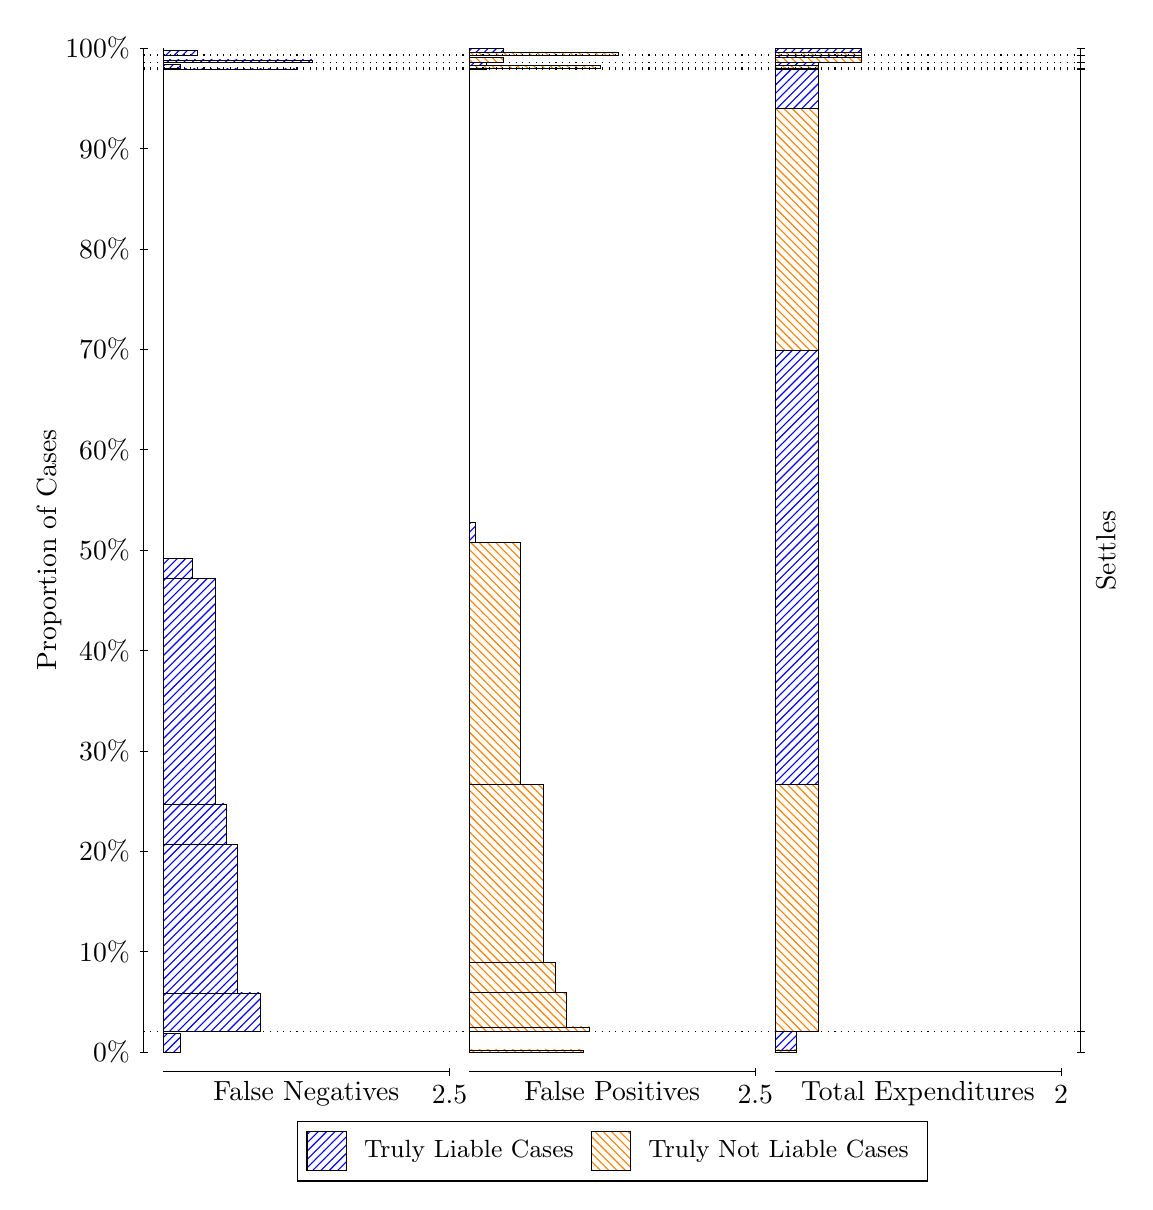
\begin{tikzpicture}
\draw[black, very thin] (1.5,1.75) -- (1.5,14.5);
\node[rotate=90, text=black, anchor=center] at (0.3, 8.125) {Proportion of Cases};
\draw[black, very thin] (1.45,1.75) -- (1.55,1.75);
\node[text=black, anchor=east] at (1.45, 1.75) {0\%};
\draw[black, very thin] (1.45,3.025) -- (1.55,3.025);
\node[text=black, anchor=east] at (1.45, 3.025) {10\%};
\draw[black, very thin] (1.45,4.3) -- (1.55,4.3);
\node[text=black, anchor=east] at (1.45, 4.3) {20\%};
\draw[black, very thin] (1.45,5.575) -- (1.55,5.575);
\node[text=black, anchor=east] at (1.45, 5.575) {30\%};
\draw[black, very thin] (1.45,6.85) -- (1.55,6.85);
\node[text=black, anchor=east] at (1.45, 6.85) {40\%};
\draw[black, very thin] (1.45,8.125) -- (1.55,8.125);
\node[text=black, anchor=east] at (1.45, 8.125) {50\%};
\draw[black, very thin] (1.45,9.4) -- (1.55,9.4);
\node[text=black, anchor=east] at (1.45, 9.4) {60\%};
\draw[black, very thin] (1.45,10.675) -- (1.55,10.675);
\node[text=black, anchor=east] at (1.45, 10.675) {70\%};
\draw[black, very thin] (1.45,11.95) -- (1.55,11.95);
\node[text=black, anchor=east] at (1.45, 11.95) {80\%};
\draw[black, very thin] (1.45,13.225) -- (1.55,13.225);
\node[text=black, anchor=east] at (1.45, 13.225) {90\%};
\draw[black, very thin] (1.45,14.5) -- (1.55,14.5);
\node[text=black, anchor=east] at (1.45, 14.5) {100\%};

\draw[black, very thin] (13.4,1.75) -- (13.4,14.5);
\draw[black, very thin] (13.35,1.75) -- (13.45,1.75);
\node[anchor=west] at (13.35, 1.75) {};
\draw[black, very thin] (13.35,2.0136) -- (13.45,2.0136);
\node[anchor=west] at (13.35, 2.0136) {};
\draw[black, very thin] (13.35,14.226) -- (13.45,14.226);
\node[anchor=west] at (13.35, 14.226) {};
\draw[black, very thin] (13.35,14.247) -- (13.45,14.247);
\node[anchor=west] at (13.35, 14.247) {};
\draw[black, very thin] (13.35,14.319) -- (13.45,14.319);
\node[anchor=west] at (13.35, 14.319) {};
\draw[black, very thin] (13.35,14.411) -- (13.45,14.411);
\node[anchor=west] at (13.35, 14.411) {};
\draw[black, very thin] (13.35,14.5) -- (13.45,14.5);
\node[anchor=west] at (13.35, 14.5) {};

\draw[black, very thin, pattern color=blue, pattern=north east lines] (1.75,1.75) rectangle (1.968,1.9858);
\draw[black, very thin, pattern color=orange, pattern=north west lines] (1.75,1.9858) rectangle (1.75,2.0136);
\draw[black, very thin, pattern color=blue, pattern=north east lines] (1.75,2.0136) rectangle (2.9853,2.5017);
\draw[black, very thin, pattern color=blue, pattern=north east lines] (1.75,2.5017) rectangle (2.6947,4.3888);
\draw[black, very thin, pattern color=blue, pattern=north east lines] (1.75,4.3888) rectangle (2.5493,4.9017);
\draw[black, very thin, pattern color=blue, pattern=north east lines] (1.75,4.9017) rectangle (2.404,7.7681);
\draw[black, very thin, pattern color=blue, pattern=north east lines] (1.75,7.7681) rectangle (2.1133,8.0139);
\draw[black, very thin, pattern color=orange, pattern=north west lines] (1.75,8.0139) rectangle (1.75,14.226);
\draw[black, very thin, pattern color=blue, pattern=north east lines] (1.75,14.226) rectangle (3.4213,14.235);
\draw[black, very thin, pattern color=orange, pattern=north west lines] (1.75,14.235) rectangle (1.75,14.247);
\draw[black, very thin, pattern color=blue, pattern=north east lines] (1.75,14.247) rectangle (1.968,14.288);
\draw[black, very thin, pattern color=orange, pattern=north west lines] (1.75,14.288) rectangle (1.75,14.319);
\draw[black, very thin, pattern color=blue, pattern=north east lines] (1.75,14.319) rectangle (3.6393,14.35);
\draw[black, very thin, pattern color=orange, pattern=north west lines] (1.75,14.35) rectangle (1.75,14.411);
\draw[black, very thin, pattern color=blue, pattern=north east lines] (1.75,14.411) rectangle (2.186,14.469);
\draw[black, very thin, pattern color=orange, pattern=north west lines] (1.75,14.469) rectangle (1.75,14.5);
\draw[black, very thin, pattern color=orange, pattern=north west lines] (5.6333,1.75) rectangle (7.0867,1.7777);
\draw[black, very thin, pattern color=blue, pattern=north east lines] (5.6333,1.7777) rectangle (5.6333,2.0136);
\draw[black, very thin, pattern color=orange, pattern=north west lines] (5.6333,2.0136) rectangle (7.1593,2.0675);
\draw[black, very thin, pattern color=orange, pattern=north west lines] (5.6333,2.0675) rectangle (6.8687,2.5086);
\draw[black, very thin, pattern color=orange, pattern=north west lines] (5.6333,2.5086) rectangle (6.7233,2.8854);
\draw[black, very thin, pattern color=orange, pattern=north west lines] (5.6333,2.8854) rectangle (6.578,5.1467);
\draw[black, very thin, pattern color=orange, pattern=north west lines] (5.6333,5.1467) rectangle (6.2873,8.2261);
\draw[black, very thin, pattern color=blue, pattern=north east lines] (5.6333,8.2261) rectangle (5.706,8.4719);
\draw[black, very thin, pattern color=blue, pattern=north east lines] (5.6333,8.4719) rectangle (5.6333,14.226);
\draw[black, very thin, pattern color=orange, pattern=north west lines] (5.6333,14.226) rectangle (5.8513,14.238);
\draw[black, very thin, pattern color=blue, pattern=north east lines] (5.6333,14.238) rectangle (5.6333,14.247);
\draw[black, very thin, pattern color=orange, pattern=north west lines] (5.6333,14.247) rectangle (7.3047,14.278);
\draw[black, very thin, pattern color=blue, pattern=north east lines] (5.6333,14.278) rectangle (5.8513,14.319);
\draw[black, very thin, pattern color=orange, pattern=north west lines] (5.6333,14.319) rectangle (6.0693,14.38);
\draw[black, very thin, pattern color=blue, pattern=north east lines] (5.6333,14.38) rectangle (5.6333,14.411);
\draw[black, very thin, pattern color=orange, pattern=north west lines] (5.6333,14.411) rectangle (7.5227,14.443);
\draw[black, very thin, pattern color=blue, pattern=north east lines] (5.6333,14.443) rectangle (6.0693,14.5);
\draw[black, very thin, pattern color=orange, pattern=north west lines] (9.5167,1.75) rectangle (9.7892,1.7777);
\draw[black, very thin, pattern color=blue, pattern=north east lines] (9.5167,1.7777) rectangle (9.7892,2.0136);
\draw[black, very thin, pattern color=orange, pattern=north west lines] (9.5167,2.0136) rectangle (10.062,5.1467);
\draw[black, very thin, pattern color=blue, pattern=north east lines] (9.5167,5.1467) rectangle (10.062,10.659);
\draw[black, very thin, pattern color=orange, pattern=north west lines] (9.5167,10.659) rectangle (10.062,13.738);
\draw[black, very thin, pattern color=blue, pattern=north east lines] (9.5167,13.738) rectangle (10.062,14.226);
\draw[black, very thin, pattern color=orange, pattern=north west lines] (9.5167,14.226) rectangle (10.062,14.238);
\draw[black, very thin, pattern color=blue, pattern=north east lines] (9.5167,14.238) rectangle (10.062,14.247);
\draw[black, very thin, pattern color=orange, pattern=north west lines] (9.5167,14.247) rectangle (10.062,14.278);
\draw[black, very thin, pattern color=blue, pattern=north east lines] (9.5167,14.278) rectangle (10.062,14.319);
\draw[black, very thin, pattern color=orange, pattern=north west lines] (9.5167,14.319) rectangle (10.607,14.38);
\draw[black, very thin, pattern color=blue, pattern=north east lines] (9.5167,14.38) rectangle (10.607,14.411);
\draw[black, very thin, pattern color=orange, pattern=north west lines] (9.5167,14.411) rectangle (10.607,14.443);
\draw[black, very thin, pattern color=blue, pattern=north east lines] (9.5167,14.443) rectangle (10.607,14.5);
\draw[black, dotted] (1.5,2.0136) -- (13.4,2.0136);
\draw[black, dotted] (1.5,14.226) -- (13.4,14.226);
\draw[black, dotted] (1.5,14.247) -- (13.4,14.247);
\draw[black, dotted] (1.5,14.319) -- (13.4,14.319);
\draw[black, dotted] (1.5,14.411) -- (13.4,14.411);
\draw[black, very thin] (1.75,1.5) -- (5.3833,1.5);
\node[text=black, anchor=north] at (3.5667, 1.5) {False Negatives};
\draw[black, very thin] (5.3833,1.45) -- (5.3833,1.55);
\node[text=black, anchor=north] at (5.3833, 1.45) {2.5};

\draw[black, very thin] (5.6333,1.5) -- (9.2667,1.5);
\node[text=black, anchor=north] at (7.45, 1.5) {False Positives};
\draw[black, very thin] (9.2667,1.45) -- (9.2667,1.55);
\node[text=black, anchor=north] at (9.2667, 1.45) {2.5};

\draw[black, very thin] (9.5167,1.5) -- (13.15,1.5);
\node[text=black, anchor=north] at (11.333, 1.5) {Total Expenditures};
\draw[black, very thin] (13.15,1.45) -- (13.15,1.55);
\node[text=black, anchor=north] at (13.15, 1.45) {2};


\node[text=black, centered, rotate=90] at (13.72, 8.12) {Settles};





\draw (7.449999999999999,1.5) node[draw=none] (baseCoordinate) {};
\begin{scope}[align=center]
        \matrix[scale=0.5, draw=black, below=0.5cm of baseCoordinate, nodes={draw}, column sep=0.1cm]{
            \node[rectangle, draw, minimum width=0.5cm, minimum height=0.5cm, pattern color=blue, pattern=north east lines] {}; &
            \node[draw=none, font=\small, text=black] (B) {Truly Liable Cases}; &
            \node[rectangle, draw, minimum width=0.5cm, minimum height=0.5cm, pattern color=orange, pattern=north west lines] {}; &
            \node[draw=none, font=\small, text=black] (B) {Truly Not Liable Cases}; \\
            };
\end{scope}

\end{tikzpicture}
\end{document}